\documentclass[10pt, conference, hidelinks, onecolumn]{IEEEtran}

\usepackage[english]{babel}
\usepackage[utf8]{inputenc}
\usepackage[cmex10]{amsmath}
\usepackage{graphicx}
\usepackage[colorinlistoftodos]{todonotes}
\usepackage{tikz}
\usepackage{fixltx2e}

\newcommand{\subparagraph}{}
\usepackage{titlesec}
\titlespacing*{\section}
{0pt}{10ex}{4ex}
\titlespacing*{\subsection}
{0pt}{4ex}{1ex}
\titlespacing*{\subsubsection}
{0pt}{4ex}{1ex}



\title{The CABS\textsubscript{score} \\ A definite video codec metric}
\author{Alberto Vigata\\ email: {\tt alberto.vigata@gmail.com}\\ \today}
\date{\today}



\usepackage{float}
\usepackage{color}
\usepackage{hyperref}
% correct bad hyphenation here
%\hyphenation{op-tical net-works semi-conduc-tor }
\usepackage{fancyhdr} % Custom headers and footers
\pagestyle{fancyplain} % Makes all pages in the document conform to the custom headers and footers
\fancyhead{} % No page header - if you want one, create it in the same way as the footers below
\fancyfoot[L]{rev 0.98} % Empty left footer
\fancyfoot[C]{} % Empty center footer
\fancyfoot[R]{} % Page numbering for right footer
\renewcommand{\headrulewidth}{0pt} % Remove header underlines
\renewcommand{\footrulewidth}{0pt} % Remove footer underlines
\setlength{\headheight}{13.6pt} % Customize the height of the header


\begin{document}



    \maketitle
    \vspace{1mm}
    \begin{abstract}
%\boldmath
    \textit{
    \noindent
Measuring video codec performance has traditionally been a simple matter. One selects an encoder and runs a sequence set through it producing the resulting compressed bitstreams. Subsequent comparisons of the size of the resulting bitstream against some chosen metric (SSIM \cite{ssim}, PSNR, ...) yields the framework for comparison of performance between different setups. While this is a valid proposition some problems are inherent with it. The lack of standardization between benchmarking setups makes their results not comparable and therefore relative. This paper introduces the $CABS_{score}$ (Codec Average Bitrate Savings) which provides a definite, clearly stated framework to the benchmarking environment.
    }
    \end{abstract}
    \vspace{3mm}



%---------------------------------
%Introduction
%---------------------------------
\section{Introduction}


\subsection{Motivation}
	With numerous video codec schemes being released frequently, the need to understand their performance characteristics is more prevalent than ever. Codec performance benchmarking is done directly by those who are releasing the product or by a third party. While results are usually shared publicly a sense of opaqueness can remain unless all the materials used during the benchmarking process are released to the public. Even when the later is available, no standardized way seems to be available to compare with other setups. $CABS_{score}$ tries to address this issue by providing a definite framework in which anyone can produce benchmarking scores and share them unambiguously with the world.

\subsection{Informal description}
$CABS_{score}$ is an intuitive and simple score, from which any reader can get a sense of the underlying performance of the codec at hand. To start with, a reference codec configuration is selected towards which all other measurements will be referred to. From this particular configuration the score calculates the codec average bitrate savings through a determined range of bitrates. The result of the score is the percentage of savings from the reference configuration.


\section{$CABS_{score}$ components}
The intent of this specification is to establish a framework in which anyone can define their own scores, and being able to share it with others in a seamless manner. In this context the specification essentially establishes the parameters surrounding the testing setup with enough specificity to remove ambiguity, and with enough flexibility to allow versatility in benchmarking scenarios. In detail a particular $CABS_{score}$ is defined with all the following required parameters:

\subsubsection{A Nickname}
\label{subsec:nickname}
The nickname of the score gets added to the subscript when referring to it. This acts as a shorthand for it. A nickname is only meaningful in the context of the other defining parameters of the score, like the sequence set, bitrage range ... Example nicknames could be '4K' for CABS\textsubscript{4K}, 'UHD' for CABS\textsubscript{UHD}


\subsubsection{A Sequence Set}
\label{subsec:sequenceset}
The specific set of uncompressed sequences that are used as input to the encoders. Such sequences must have the same resolution $\mathcal{S}$ but they can vary in the frame count.


\subsubsection{A Bitrate Range}
\label{subsec:bitraterange}
The range of bitrates $\lbrace br_{low} \to br_{high} \rbrace $ where the score is going to be performed and where the RD curves are going to be evaluated


\subsubsection{A Reference Codec Configuration}
\label{subsec:refcodecconfig}
The reference RD curve that all the other curves are compared to. This can be defined through a specific configuration for an encoder or providing the encoded bitstreams of the encoded configuration


\subsubsection{A Frame based metric used for comparison}
\label{subsec:framebasemetric}
The specific metric used for measuring the distortion introduced by the coded due to the encoding process. For example SSIM or PSNR. Pseudo-code or equivalent algorithmic description must be provided to instruct how to derive the metric numbers on a frame by frame basis.

\subsection{NOTES}
All this parameters must be provided along side the score for it to be valid. However, the general goal is that a specific nickname will be generally known to be equivalent to all the other parameters as a short hand. For example $CABS_{4KvsHD1}$ could be used as the nickname for one specific set of parameters available in some public repository, such specific $CABS_{score}$ would measure performance of codecs on 4K video compared to an HD era video codec.

\subsubsection{Materials distribution}
The particular way in which the components of a $CABS_{score}$ are distributed are beyond the scope of this specification. However, here are a few suggestions:

\begin{itemize}
  \item The sequence set (see~\ref{subsec:sequenceset}) can be provided as a set of files along with their SHA-1 hashes\cite{shs} to verify their signature
  \item The reference binaries used to produce the reference bitstream (see~\ref{subsec:refcodecconfig}) can be provided precompiled for a specific platform, along side with exact configuration files that produce the reference bitstreams. Alternatively, just the reference bitstreams can be provided as they can be decoded with the video decoder under study, and resulting reference RD curves can be derived from it given the availability of~\ref{subsec:sequenceset}
  \item Specific implementations of frame-based metrics like SSIM or PSNR must be provided. It is suggested that alongside reference code that produces the reference metric results, the resulting metric values for the sequence set in~\ref{subsec:sequenceset} are provided. For example, if metric is SSIM based, the values that this particular SSIM implementation metric produces on~\ref{subsec:sequenceset} can be provided for validation purposes.
\end{itemize}


\section{Calculation}
The following steps must be followed to produce a $CABS_{score}$ that is complaint with this spec:
\subsection{RD Curve sampling}
Due to the intrinsic non-linear nature of the rate distortion curve for a specific codec configuration, the RD curve must be empirically sampled. This specification requires that the RD curve is sampled with a density of at least 10 points through the bitrate range of coverage. For example if the bitrate range is $\lbrace 500_{kbps} \to 2500_{kbps} \rbrace $ a encoded bitstream must be obtained per configuration with resulting bitrate every $200_{kbps}$ for the range.


\subsection{RD Curve interpolation}
In order to extrapolate values outside the sampled RD curve in the previous step, linear interpolation between the sampled points must be used. The resulting function $ref(x)$ corresponds to the mathematical extrapolated representation of the RD curve. Figure~\ref{fig:x264rd} shows a sampled RD curve for the x264 100-2500kbps for the PSNR metric. While other types of interpolation maybe possible, linear interpolation is chosen for its simplicity.

\begin{figure}[!ht]
\centering
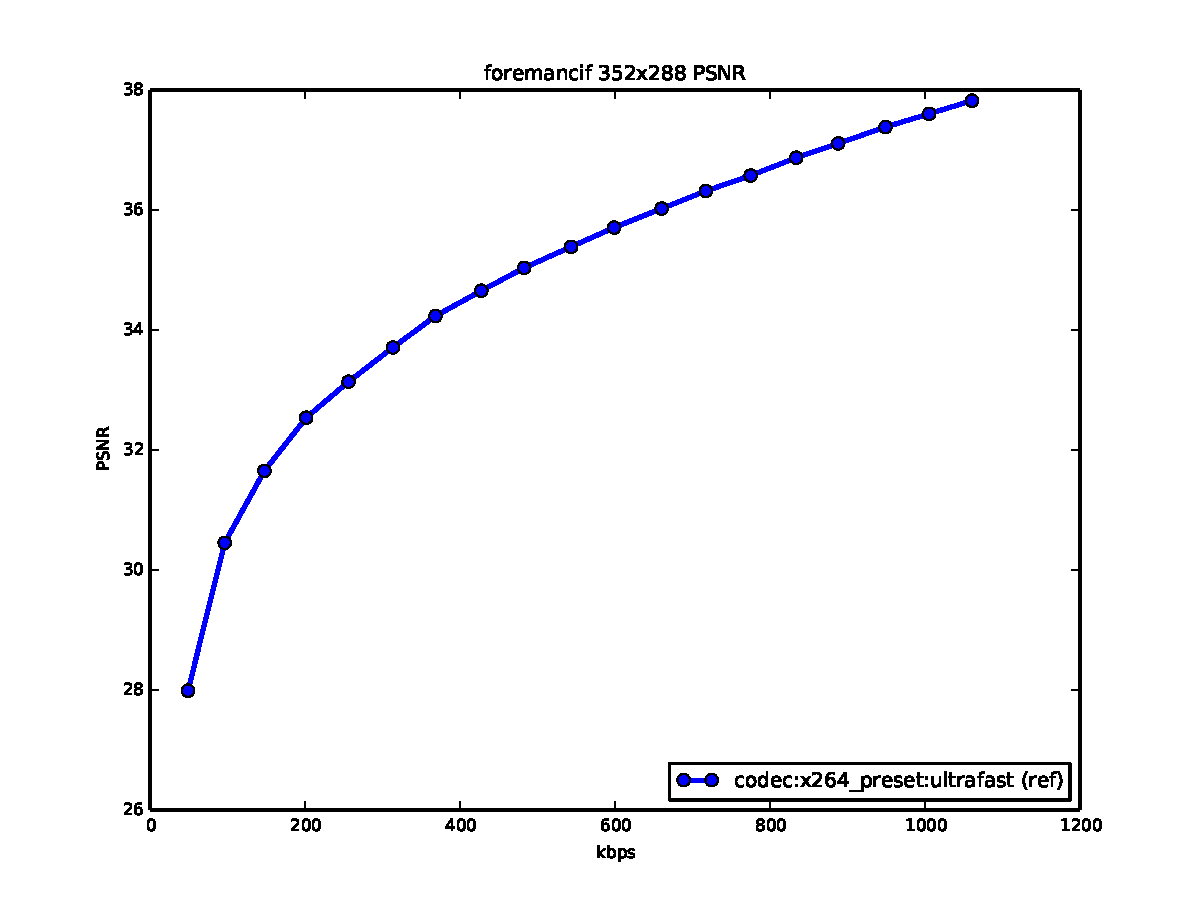
\includegraphics[width=3.8in,height=2.3in]{x264_rd}
\caption{x264 RD curve for foreman CIF, medium preset, from 100kbps to 2000kpbs, PSNR}
\label{fig:x264rd}
\end{figure}

\subsection{Determine Metric range from the bitrate reference range for a specific sequence}
The Average Bitrate Savings is informally defined as the average distance in bitrate between the reference RD curve $ref(x)$ and the testing curve $g(x)$. The average distance is calculated in the y axis (the metric axis) between two points: a lower $M_{low}$ and a higher $M_{high}$. Both points are formally derived from the reference curve as follows: 

\begin{gather}
M_{low} = ref(br_{low})\\
M_{high} = ref(br_{high})
\end{gather}
\vskip 2ex

\subsection{Calculate bitrate RD Curve differentiation for a specific sequence}
In order to find the average distance between the reference RD curve $ref(x)$ and the measuring curve $g(x)$ we measure such distance on a $N$ number of points on the extrapolated curves and then we produce the average. N must be greater or equal than 10000. More formally:
\begin{equation}
step = \frac{M_{high}-M_{low}}{N}
\end{equation}
\begin{equation}
y_k = step\cdot k+M_{low}
\end{equation}
\begin{equation}
AverageBitrateSavings_{score_{seqi}}=
\frac{1}{N}\sum_{k=0}^{N}\frac{ref^{-1}(y_k)-g^{-1}(y_k)}{ref^{-1}(y_k)}
\end{equation}
\vskip 2ex

\subsection{Average over sequences}
To obtain the final score, we average the $ABS_{score}$ over multiple sequences to obtain the final $CABS_{score}$
\begin{equation}
CABS_{score} = \sum AverageBitrateSavings_{score_{seqi}}
\end{equation}


\begin{thebibliography}{9}
\bibitem{ssim}
Zhou Wang,
Alan C. Bovik, 
Hamid R. Sheikh and Eero P. Simoncelli
\emph{The SSIM Index for Image Quality Assessment  \\https://ece.uwaterloo.ca/~z70wang/research/ssim/}

\bibitem{shs}
FEDERAL INFORMATION PROCESSING STANDARDS PUBLICATION
\emph{Secure Hash Standard \\http://csrc.nist.gov/publications/fips/fips180-4/fips-180-4.pdf}

\end{thebibliography}

\end{document}
